\documentclass[11pt]{article}
\input{\string~/.preamble}
\geometry{margin=0.5in}

\DeclareUrlCommand\uscore{\urlstyle{rm}}

% arg1=pdfurl arg2=pagenum arg3=text
\newcommand{\linkpaper}[3][.]{
    \noindent\href[page=#2]{#1}{\uscore{#3}}
} 
\newcommand{\bx}{\mathbf{x}}
\renewcommand{\argmax}{\arg\!\max}


\setlist[itemize]{noitemsep, topsep=0pt}

\begin{document}

\tableofcontents
\newpage

\section{Color CFA Demosaicing}

\subsection{
    \linkpaper[../papers/2005_demosaicking_color_filter_array_interpolation.pdf]{1}{2005_demosaicking_color_filter_array_interpolation}
}

\begin{itemize}
    \item \textbf{color filter array (CFA)} are filters that allow only 1 color to be measured at each pixel
    \item \textbf{demosaiking} is the process of estimating 2 missing colors at each pixel 
    \item \textbf{Non-adaptive Interpolation}
    \begin{itemize}
        \item \textbf{bilinear interpolation} perform linear interpolation in one direction, then again in the other direction. The interpolation is quadratic overall.
        \[
            f(x, y) = \sum_{i=0}^1 \sum_{j=0}^1 a_{ij} \bx^{i} \bx^{j}
        \]
        \item \textbf{splines} (\href{https://en.wikipedia.org/wiki/Spline_(mathematics)#Definition}{wiki}) is a function consists of piecewise polynomials $S:[a,b] \to \R$. Given $k+1$ coordinates, there are algorithms for finding $k$ polynomials that ensures continuity, smoothness, etc. Can be used for data interpolation. 
        \item \textbf{cubic hermite splines} is a spline where each piece is 3rd degree polynomial in hermit form. Inputs points and tangents at the points, where tangents maybe approximated from neighborhing points.
        \item \textbf{bicubic interpolation} Extension of cubic hermite splines for interpolating data points on 2d grids. Resulting surface smoother than bilinear interpolation. Determine coefficients $a_{ij}$ from values of nearby pixels
        \[
            f(x, y) = \sum_{i=0}^3 \sum_{j=0}^3 a_{ij} \bx^{i} \bx^{j}
        \]
    \end{itemize}
    \item \textbf{Heuristic-based Interpolation} filtering operations based on reasonable assumptions
    \begin{itemize}
        \item \textbf{edge-directed interpolation} edge direction is estimated first to avoid interpolating across edges, then the missing sample is estimated by interpolating alone the edge. The preferred interpolation direction has a smaller gradient.
        \item \textbf{constant-hue interpolation} interpolates G channel using edge-directed interpolation, and R,B channels estimated from the interpolated R hue (R-to-G ratio) and B hue (B-to-G ratio). The assumption is hue is within an object in an image is constant, regardless of varying lighting condition. This assumes perfect interchannel correlation.
        \item \textbf{weighted average interpolation} defines edge indicators in several directions as measures of edge likelihood in those directions and determines missing pixel intensity as a weighted sum of its neighbors.
        \item \textbf{second-order gradients as correction terms} reduce aliasing for edge-directed interpolation
        \item \textbf{alias canceling interpolation} 
        \item \textbf{homogeneity-directed interpolation} Use local homogeneity as an indicator to choose between horizontally and vertically interpolated intensities. Local homogeneity is measured by the total number of similar luminance and chrominance values of the pixels that are within a neighborhood of the pixel. 
        \item \textbf{pattern matching} find a pttern in data and fit data to one of the template, then apply different interpolators to each template, i.e. different interpolation for edges and/or smooth regions.
        \item \textbf{vector-based interpolation} Each pixel as a vector in 3d space, interpolation is treated as minimizing the angle or distance among the neighboring vectors. For example, enforce similar chrominance values locally.
    \end{itemize}
    \item \textbf{Reconstruction-based Interpolation} makes assumption about interchannel correlation or priors and solve an optimization problem based on these assumptions
    \begin{itemize}
        \item \textbf{regularization} minimizes iteratively a cost function consisting of a spatical smoothness and a color correlation term
        \item \textbf{projections onto convex sets} 
        \item \textbf{bayesian approach} incorporates priors (spatial smoothness and constant color ratio) and noise statistics into solution. 
        \[
            \hat{S} = \argmax_{S} \{ p(S|O)\} = \argmax_{S} \{ p(O|S)p(S)\} 
        \]
        where observed data $O$, color channels $S$, and additive noises $N$ are treated as random variables. The solution maximizes posterior probability (MAP)
        \item \textbf{artifical neural networks} weights learnt from training data. 
    \end{itemize}
    \item \textbf{Image Formation Modeling} fomulate demosaiking as an inverse problem (calculating causal source) accounting for colorf filters, lens distortions, sensor noise and determine most likely output given measured CFA images. Given a model for image formation
    \[
        \mathbf{O} = \mathbf{Hr + N}
    \]
    find radiance $\mathbf{r}$
    \item \textbf{experiments} 
    \begin{itemize}
        \item 24 test color images
        \item metrics
        \begin{itemize}
            \item MSE
            \item Spatial-CIELAB, measuring quality of color reconstruction in a perceptually uniform color space.
            \item a measure of zipper effect
            \item subjective viewing
        \end{itemize}
        \item POCS (projection onto convex set) method performs the best under MSE. Homogeneity-directed interpolation reconstructs image best subjectively (no aliasing).
    \end{itemize}
\end{itemize}


\subsection{
    \linkpaper[../papers/2008_image_demosaicing_a_systematic_survey.pdf]{1}{2008_image_demosaicing_a_systematic_survey}
}

\begin{itemize}
    \item \textbf{problem formulation} Denote full-resolution color image as $S=(R,G,B)$ and bayer pattern as $z_S = (z_R, z_G, z_B)$. 
    \begin{itemize}
        \item \textbf{statistical} Bayesian framework
        \[
            P(S|z_S, \mathcal{H}) = 
            \frac{
                P(z_S | S, \mathcal{H}) p(S|\mathcal{H})
            }{
                P(z_S | \mathcal{H})
            }
        \]
        where $\mathcal{H}$ is the assumed model. the likelihood represents the imaging model. the prior $p(S|\mathcal{H})$ captures spatial-spectral correlation. We can decompose
        \[
            p(S) = p(G) p(R,B | G)
            = p(G) p(R|G) p(B|G)
            = p(G) p(R-G) p(B-G)
        \]
        where the latter two terms represent inter-channel differences. This model is called sequential inter-channel model.
        \item \textbf{deterministic in frequency domain} View mosaiced data $z$ as a down-sampling from $S$.
        \[
            z = \sum_{S\in\{R,G,B\}} z_S = \sum_{S\in \{R,G,B\}} M_S S
        \]
        where $z$ are subsampled color channels and the mask $M_S$ takes a color sample at a pixel according to bayer CFA pattern, i.e. at a red pixel $M_R = 1$, $M_G = 0$, and $M_B = 0$. The masks for bayer CFA can be written as a function of cosines.
        \begin{align*}
            M_R(i,j) &= \frac{1}{4} (1-\cos{\pi i}) (i+\cos{\pi j}) \\
            M_G(i,j) &= \frac{1}{2} (1 + \cos{\pi i} \cos{\pi j}) \\
            M_B(i, j) &= \frac{1}{4} (1 + \cos{\pi i})(1 - \cos{\pi j}) \\ 
        \end{align*}
    \end{itemize}
    \item \textbf{standard interpolation methods} bilinear/cubic interpolation, spline interpolation treat each channes separately without utilizing inter-channel correlation.
    \item \textbf{sequential demosaicing methods} 
    \begin{itemize}
        \item \textbf{idea} luminance (G) channel is less alised than the other two (B,R). Idea is to interpolate $G$ channels first then interpolate the other two.
        \item \textbf{luminance (green) channel interpolation} with heuristic edge-directed interpolation methods in the frequency domain. Or recovering in the frequency domain.
        \item \textbf{chrominance (red/blue) channel interpolation} based on assumption that hue (color ratios or differences) is constant wihtin boundary of objects. This assumption works less well for higher quality dataset. 
        \item \textbf{refinement techniques} used to mediate artifacts (false color, zipper, etc.). Median filtering, etc.
        \item \textbf{problems} errors rendered during interpolation of luminance (G) channel is propagated to the chrominance channels. This can be alleviated by iterative optimization.
    \end{itemize}
    \item \textbf{learning-based methods} learn the relationship between CFA pattern and the surrounding pixels.
    \item \textbf{performance evaluation}
    \begin{itemize}
        \item mean squared error (MSE) or equivalently peak signal to noise ratio (PSNR) 
        \item mean absolute difference (MAD) and normalized color difference (NCD)
        \item euclidean distance in perceptually uniform CIELab spaces and s-CIELab
    \end{itemize}
    \item \textbf{experimental results}
    \begin{itemize}
        \item 11 inter-channel demosaicing algorithms \linkpaper[../papers/2008_image_demosaicing_a_systematic_survey.pdf]{13}{references}
        \begin{center}
            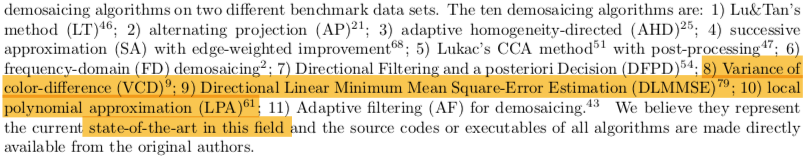
\includegraphics[width=0.8\textwidth]{images/2008_survey_1.png}
        \end{center}
        \item 2 benchmark dataset: KodaK PhotoCD (512$\times$768) and IMAX high-quality images (4M)
        \item 2 metrics: PSNR and S-CIELab measure.
        \item take away: important to jointly exploiting spatial and spectral correlations for images with high saturation and varying-hue. Constant-hue assumption fails for algorithms that rely on them, and so performs worse on the more difficult IMAX image dataset. Also the performance are quite good close to each other.
        \item For Kodak dataset 
        \begin{itemize}
            \item 2006 Color demosaicing using variance of color differences.
            \item 2005 Color demosaicking via directional linear minimum mean square-error estimation.
            \item 2007 Spatially adaptive color filter array interpolation for noiseless and noisy data.
        \end{itemize}
        \item For IMAX dataset, constant-hue assumption breaks down ...
        \begin{itemize}
            \item 2001 New edge directed interpolation (NEDI: intra-channel approach)
            \item 2007 Adaptive filtering for color filter array demosaicking.
        \end{itemize}
    \end{itemize}
\end{itemize}
 
\subsection{
    \linkpaper[../papers/2011_color_image_demosaicking_an_overview.pdf]{1}{2011_color_image_demosaicking_an_overview}
}

\begin{itemize}
    \item \textbf{heuristic methods} assumes hue is smoother than color within boundaries. So interpolate G channel first, then recosntruct R, B by interpolation of color ratio/differences. Adaptive methods based on first determine the direction for interpolation to avoid interpolating cross edges.
    \item \textbf{directional interpolation} interpolate along vertical and horizontal directions, and pick the better one a posteriori.
    \item \textbf{frequency domain} 
    \item \textbf{Quality Assessment}
    \begin{itemize}
        \item \textbf{means square error (MSE)}
        \[
            MSE(X) = \frac{1}{N_1 N_2} \sum_{n_1=1}^{N_1} \sum_{n_2=1}^{N_2} 
            \left(
                \hat{X}(n_1, n_2) - X(n_1, n_2)
            \right)^2
            \qquad
            X \in \{R, G, B\}
        \]
        where $X$ represent each of 3 color channels. 
        \item \textbf{(color) peak Signal-to-noise ratio (CPSNR)}
        \[
            CPSNR = 10 \log_{10} \frac{255^2}{\frac{1}{3} \sum_{X\in \{R,G,B\}} MSE(X)}
        \]
        \item \textbf{S-CIELAB} quantify performance catered to human percecption 
        \item \textbf{visual inspection} in detailed regions
    \end{itemize}
    \item \textbf{Results} 19, 38, 75 has good performance. Good performance from directional approaches. Good to analyze dmosaiking jointly with zooming, denoising, super-resolution. 
    \begin{itemize}
        \item 19: 2006 Color demosaicing using variance of color differences. (good PSNR, good S-CIELAB, almost no zipper)
        \item 38: 2007 Demosaicing based on wavelet analysis of the luminance component. 
        \item 75: 2008 Sparse representation for color image restoration 
    \end{itemize}
\end{itemize}



\section{Related to the project}

\subsection{
    \linkpaper[../papers/2018_coded_two_bucket_cameras_for_computer_vision.pdf]{1}{2018_coded_two_bucket_cameras_for_computer_vision}
}


\begin{itemize}
    \item \textbf{abstract} 
\end{itemize}


\section{Terminologies}

\begin{enumerate}
    \item \textbf{photometric stereo} \href{https://en.wikipedia.org/wiki/Photometric_stereo}{wiki} technique for estimating surface normal by observing objects under different lighting conditions
    \item \textbf{albedo} \href{https://en.wikipedia.org/wiki/Albedo}{wiki} is the measure of the diffuse reflection of solar radiation out of the total solar radiation received by an astronomical body, scales from 0 (absorbs all light) to 1 (reflects all light).
\end{enumerate}


\end{document}
